\noindent O primeiro exemplo escolhido foi com a função \(f_1(x) = \sin(x) - \exp(x)\). O código seguinte permite constuir a tabela respetiva e o gráfico:

\lstinputlisting{II/f1.m}
O gráfico e a tabela obtidos são os seguintes:

\begin{figure}[ht]
    \centering
    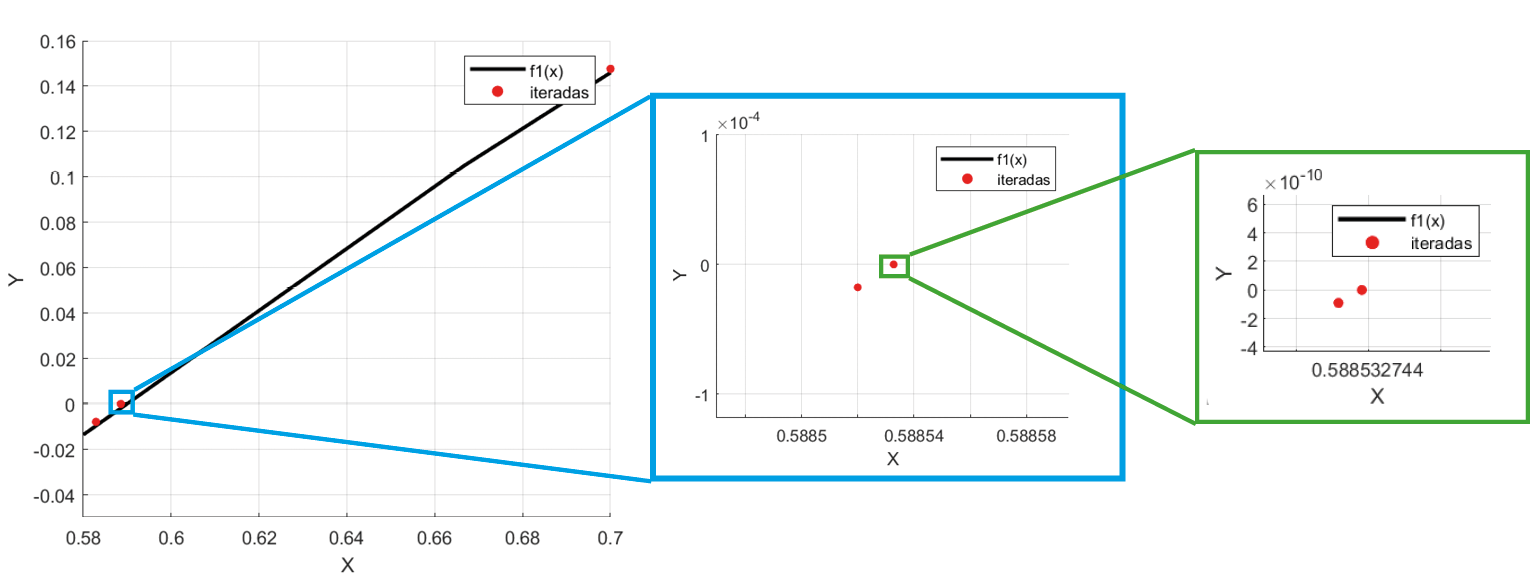
\includegraphics[width=\textwidth]{II/grafico_f1.png}
    \label{grafico_f1}
\end{figure}

\begin{table}[ht]
    \centering
    \begin{tabular}{|c|c|c|c|c|c|}
    \hline
    \(n\) & \(x_n\) & \(|e_n|\) & \(\displaystyle \frac{|e_{n+1}|}{|e_n|}\) & \(\displaystyle \frac{|e_{n+1}|}{|e_n|^2}\) & \(\displaystyle \frac{|e_{n+1}|}{|e_n|^3}\) \\
    \hline
    0 & $0.700000000000000$ & $0.111467$                 & $0.050765$                & $0.455432$ & $4.08579$ \\
    1 & $0.582874018545673$ & $0.005658$                 & $0.002250$                & $0.397736$ & $70.2872$ \\
    2 & $0.588520007998022$ & $1.273598 \times 10^{-5}$  & $5.097818 \times 10^{-6}$ & $0.400268$ & $3.14281 \times 10^4$ \\
    3 & $0.588532743916935$ & $6.492573 \times 10^{-11}$ & & & \\
    4 & $0.588532743981861$ & & & & \\
    \hline
    \multicolumn{6}{|c|}{$p = 2\quad K_{\infty} \approx 0.4$}\\
    \hline
    \end{tabular}
\end{table}

\noindent Pelo gráfico percebe-se que, de facto, as iteradas estão a convergir para \(z\). Apesar do reduzido número de iteradas, os valores da tabela permitem concluir que \(\displaystyle \frac{|e_{n+1}|}{|e_n|}\) deve convergir para 0 e \(\displaystyle \frac{|e_{n+1}|}{|e_n|^3}\) deve convergir para \(\infty\). Já os valores \(\displaystyle \frac{|e_{n+1}|}{|e_n|^2}\) devem convergir para um \(K_\infty \approx 0.4\), mostrando a convergência de ordem 2.